\documentclass{tufte-handout}

\title{CS224n: Natural Language Processing with Deep Learning\thanks{Course Instructors: Christopher Manning, Richard Socher}}

\author[Rohit Mundra, Richard Socher]{Lecture Notes: Part II\thanks{Author: Rohit Mundra, Emma Peng, Richard Socher, Ajay Sohmshetty}}

\date{Winter 2017} % without \date command, current date is supplied

%\geometry{showframe} % display margins for debugging page layout

\usepackage{graphicx} % allow embedded images
  \setkeys{Gin}{width=\linewidth,totalheight=\textheight,keepaspectratio}
  \graphicspath{{notes2/fig/}} % set of paths to search for images
\usepackage{amsmath}  % extended mathematics
\usepackage{amstext}  % extended text
\usepackage{booktabs} % book-quality tables
\usepackage{units}    % non-stacked fractions and better unit spacing
\usepackage{multicol} % multiple column layout facilities
\usepackage{lipsum}   % filler text
\usepackage{fancyvrb} % extended verbatim environments
\usepackage{placeins}
  \fvset{fontsize=\normalsize}% default font size for fancy-verbatim environments

% Standardize command font styles and environments
\newcommand{\doccmd}[1]{\texttt{\textbackslash#1}}% command name -- adds backslash automatically
\newcommand{\docopt}[1]{\ensuremath{\langle}\textrm{\textit{#1}}\ensuremath{\rangle}}% optional command argument
\newcommand{\docarg}[1]{\textrm{\textit{#1}}}% (required) command argument
\newcommand{\docenv}[1]{\textsf{#1}}% environment name
\newcommand{\docpkg}[1]{\texttt{#1}}% package name
\newcommand{\doccls}[1]{\texttt{#1}}% document class name
\newcommand{\docclsopt}[1]{\texttt{#1}}% document class option name
\newenvironment{docspec}{\begin{quote}\noindent}{\end{quote}}% command specification environment
\newcommand{\argmin}{\operatornamewithlimits{argmin}}
\newcommand{\argmax}{\operatornamewithlimits{argmax}}
\newcommand{\textunderscript}[1]{$_{\text{#1}}$}

\setcounter{secnumdepth}{3}

\begin{document}

\maketitle% this prints the handout title, author, and date

%\printclassoptions


\textbf{Keyphrases: Global Vectors for Word Representation (GloVe). Intrinsic and extrinsic evaluations. Effect of hyperparameters on analogy evaluation tasks. Correlation of human judgment with word vector distances. Dealing with ambiguity in word using contexts. Window classification.}

This set of notes first introduces the GloVe model for training word vectors. Then it extends our discussion of word vectors (interchangeably called word embeddings) by seeing how they can be evaluated intrinsically and extrinsically. As we proceed, we discuss the example of word analogies as an intrinsic evaluation technique and how it can be used to tune word embedding techniques. We then discuss training model weights/parameters and word vectors for extrinsic tasks. Lastly we motivate artificial neural networks as a class of models for natural language processing tasks.

\section[GloVe]{Global Vectors for Word Representation (GloVe)\footnote{This section is based on the GloVe paper by Pennington et al.: \\ Jeffrey Pennington, Richard Socher, and Christopher D. Manning. 2014. GloVe: Global Vectors for Word Representation}}

\subsection{Comparison with Previous Methods}
So far, we have looked at two main classes of methods to find word embeddings. The first set are count-based and rely on matrix factorization (e.g. LSA, HAL). While these methods effectively leverage global statistical information, they are primarily used to capture word similarities and do poorly on tasks such as word analogy, indicating a sub-optimal vector space structure. 
The other set of methods are shallow window-based (e.g. the skip-gram and the CBOW models), which learn word embeddings by making predictions in local context windows. These models demonstrate the capacity to capture complex linguistic patterns beyond word similarity, but fail to make use of the global co-occurrence statistics.

\marginnote{\textbf{GloVe:}
\begin{itemize}
\item Using global statistics to predict the probability of word j appearing in the context of word i with a least squares objective
\end{itemize}
}

In comparison, GloVe consists of a weighted least squares model that trains on global word-word co-occurrence counts and thus makes efficient use of statistics. The model produces a word vector space with meaningful sub-structure. It shows state-of-the-art performance on the word analogy task, and outperforms other current methods on several word similarity tasks.

\subsection{Co-occurrence Matrix}

\marginnote{\textbf{Co-occurrence Matrix:}
\begin{itemize}
\item $X$: word-word co-occurrence matrix
\item $X_{ij}$: number of times word $j$ occur in the context of word $i$
\item $X_i = \sum_k X_{ik}$: the number of times any word k appears in the context of word i
\item $P_{ij} = P(w_j | w_i) = \frac{X_{ij}}{X_i}$: the probability of j appearing in the context of word i
\end{itemize}
}

Let $X$ denote the word-word co-occurrence matrix, where $X_{ij}$ indicates the number of times word $j$ occur in the context of word $i$. Let $X_i = \sum_k X_{ik}$ be the number of times any word k appears in the context of word i. Finally, let $P_{ij} = P(w_j | w_i) = \frac{X_{ij}}{X_i}$ be the probability of j appearing in the context of word i.

Populating this matrix requires a single pass through the entire corpus to collect the statistics. For large corpora, this pass can be computationally expensive, but it is a one-time up-front cost.

\subsection{Least Squares Objective}
Recall that for the skip-gram model, we use softmax to compute the probability of word j appears in the context of word i:

\[
	Q_{ij} = \frac{\exp(\vec{u}_j^T \vec{v}_i)}{\sum_{w=1}^W \exp(\vec{u}_w^T \vec{v}_i)}
\]

Training proceeds in an on-line, stochastic fashion, but the implied global cross-entropy loss can be calculated as:

\[
	J = -\sum_{i \in corpus} \sum_{j \in context(i)} \log Q_{ij}
\]

As the same words i and j can appear multiple times in the corpus, it is more efficient to first group together the same values for i and j:

\[
	J = -\sum_{i=1}^W \sum_{j=1}^W X_{ij} \log Q_{ij}
\]

where the value of co-occurring frequency is given by the co-occurrence matrix $X$. One significant drawback of the cross-entropy loss is that it requires the distribution $Q$ to be properly normalized, which involves the expensive summation over the entire vocabulary. Instead, we use a least square objective in which the normalization factors in $P$ and $Q$ are discarded:

\[
	\hat{J} = \sum_{i=1}^W \sum_{j=1}^W X_i (\hat{P}_{ij} - \hat{Q}_{ij})^2
\]

where $\hat{P}_{ij} = X_{ij}$ and $\hat{Q}_{ij} = \exp(\vec{u}_j^T \vec{v}_i)$ are the unnormalized distributions. This formulation introduces a new problem -- $X_{ij}$ often takes on very large values and makes the optimization difficult. An effective change is to minimize the squared error of the logarithms of  $\hat{P}$ and $\hat{Q}$:

\begin{align*}
	\hat{J} & = \sum_{i=1}^W \sum_{j=1}^W X_i (\log(\hat{P})_{ij} - \log(\hat{Q}_{ij}))^2 \\
    & = \sum_{i=1}^W \sum_{j=1}^W X_i (\vec{u}_j^T \vec{v}_i - \log X_{ij})^2
\end{align*}

Another observation is that the weighting factor $X_i$ is not guaranteed to be optimal. Instead, we introduce a more general weighting function, which we are free to take to depend on the context word as well:

\[
	\hat{J} = \sum_{i=1}^W \sum_{j=1}^W f(X_{ij}) (\vec{u}_j^T \vec{v}_i - \log X_{ij})^2
\]

\subsection{Conclusion}
In conclusion, the GloVe model efficiently leverages global statistical information by training only on the nonzero elements in a word-word co-occurrence matrix, and produces a vector space with meaningful sub-structure. It consistently outperforms $word2vec$ on the word analogy task, given the same corpus, vocabulary, window size, and training time. It achieves better results faster, and also obtains the best results irrespective of speed. 


\section{Evaluation of Word Vectors}\label{sec:eval-wv}

So far, we have discussed methods such as the \textit{Word2Vec} and \textit{GloVe} methods to train and discover latent vector representations of natural language words in a semantic space. In this section, we discuss how we can quantitatively evaluate the quality of word vectors produced by such techniques.

\subsection{Intrinsic Evaluation}\label{sec:intrinsic}
Intrinsic evaluation of word vectors is the evaluation of a set of word vectors generated by an embedding technique (such as Word2Vec or GloVe) on specific intermediate subtasks (such as analogy completion). These subtasks are typically simple and fast to compute and thereby allow us to help understand the system used to generate the word vectors. An intrinsic evaluation should typically return to us a number that indicates the performance of those word vectors on the evaluation subtask. 

\begin{marginfigure}%
  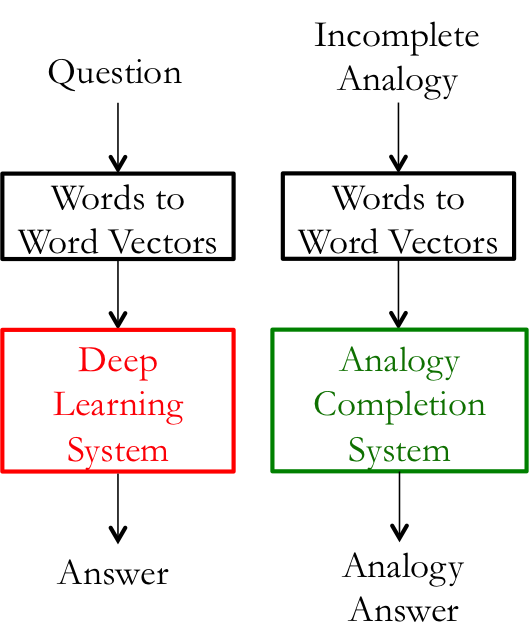
\includegraphics[width=\linewidth]{IntrinsicEval}
  \caption{The left subsystem (red) being expensive to train is modified by substituting with a simpler subsystem (green) for intrinsic evaluation.}
  \label{fig:IntrinsicEval}
\end{marginfigure}

\textbf{Motivation:} Let us consider an example where our final goal is to create a question answering system which uses word vectors as inputs. One approach of doing so would be to train a machine learning system that:
\begin {enumerate}
\item Takes words as inputs
\item Converts them to word vectors
\item Uses word vectors as inputs for an elaborate machine learning system
\item Maps the output word vectors by this system back to natural language words
\item Produces words as answers
\end{enumerate}

\marginnote{\textbf{Intrinsic evaluation:}
\begin{itemize}
\item Evaluation on a specific, intermediate task
\item Fast to compute performance
\item Helps understand subsystem
\item Needs positive correlation with real task to determine usefulness
\end{itemize}
}

Of course, in the process of making such a state-of-the-art question-answering system, we will need to create optimal word-vector representations since they are used in downstream subsystems (such as deep neural networks). To do this in practice, we will need to tune many hyperparameters in the Word2Vec subsystem (such as the dimension of the word vector representation). While the idealistic approach is to retrain the entire system after any parametric changes in the Word2Vec subsystem, this is impractical from an engineering standpoint because the machine learning system (in step 3) is typically a deep neural network with millions of parameters that takes very long to train. In such a situation, we would want to come up with a simple intrinsic evaluation technique which can provide a measure of "goodness" of the word to word vector subsystem. Obviously, a requirement is that the intrinsic evaluation has a positive correlation with the final task performance.

\subsection{Extrinsic Evaluation}\label{sec:extrinsic}

\marginnote{\textbf{Extrinsic evaluation:}
\begin{itemize}
\item Is the evaluation on a real task
\item Can be slow to compute performance
\item Unclear if subsystem is the problem, other subsystems, or internal interactions
\item If replacing subsystem improves performance, the change is likely good
\end{itemize}
}

Extrinsic evaluation of word vectors is the evaluation of a set of word vectors generated by an embedding technique on the real task at hand. These tasks are typically elaborate and slow to compute. Using our example from above, the system which allows for the evaluation of answers from questions is the extrinsic evaluation system. Typically, optimizing over an underperforming extrinsic evaluation system does not allow us to determine which specific subsystem is at fault and this motivates the need for intrinsic evaluation.

\subsection{Intrinsic Evaluation Example: Word Vector Analogies}
A popular choice for intrinsic evaluation of word vectors is its performance in completing word vector analogies. In a word vector analogy, we are given an incomplete analogy of the form:\\
\centerline{a : b : : c : ?}
The intrinsic evaluation system then identifies the word vector which maximizes the cosine similarity:
$$ d = \argmax_i \frac{(x_b - x_a + x_c)^Tx_i} {\|x_b - x_a + x_c\|}$$
This metric has an intuitive interpretation. Ideally, we want $x_b - x_a = x_d - x_c$ (For instance, queen -- king = actress -- actor). This implies that we want $x_b - x_a + x_c = x_d$. Thus we identify the vector $x_d$ which maximizes the normalized dot-product between the two word
vectors (i.e. cosine similarity).

Using intrinsic evaluation techniques such as word-vector analogies should be handled with care (keeping in mind various aspects of the corpus used for pre-training). For instance, consider analogies of the form:\\
\centerline{City 1 : State containing City 1 : : City 2 : State containing City 2}

\begin{table}[ht]
  \centering
  \fontfamily{ppl}\selectfont
  \begin{tabular}{ll}
    \toprule
    Input & Result Produced \\
    \midrule
    Chicago : Illinois : : Houston & Texas\\
    Chicago : Illinois : : Philadelphia & Pennsylvania \\
    Chicago : Illinois : : Phoenix & Arizona\\
    Chicago : Illinois : : Dallas & Texas\\
    Chicago : Illinois : : Jacksonville & Florida \\
    Chicago : Illinois : : Indianapolis & Indiana \\
    Chicago : Illinois : : Austin & Texas\\
    Chicago : Illinois : : Detroit & Michigan\\
    Chicago : Illinois : : Memphis & Tennessee \\
    Chicago : Illinois : : Boston & Massachusetts\\
    \bottomrule
  \end{tabular}
  \caption{Here are \textbf{semantic} word vector analogies (intrinsic evaluation) that may suffer from different cities having the same name}
  \label{tab:normaltab}
\end{table}

In many cases above, there are multiple cities/towns/villages with the same name across the US. Thus, many states would qualify as the right answer. For instance, there are at least 10 places in the US called Phoenix and thus, Arizona need not be the only correct response. Let us now consider analogies of the form:\\
\centerline{Capital City 1 : Country 1 : : Capital City 2 : Country 2}

\begin{table}[ht]
  \centering
  \fontfamily{ppl}\selectfont
  \begin{tabular}{ll}
    \toprule
    Input & Result Produced \\
    \midrule
	Abuja : Nigeria : : Accra & Ghana\\
	Abuja : Nigeria : : Algiers & Algeria\\
	Abuja : Nigeria : : Amman & Jordan\\
	Abuja : Nigeria : : Ankara & Turkey\\
	Abuja : Nigeria : : Antananarivo & Madagascar \\
	Abuja : Nigeria : : Apia & Samoa\\
	Abuja : Nigeria : : Ashgabat & Turkmenistan \\
	Abuja : Nigeria : : Asmara & Eritrea\\
	Abuja : Nigeria : : Astana & Kazakhstan\\
    \bottomrule
  \end{tabular}
  \caption{Here are \textbf{semantic} word vector analogies (intrinsic evaluation) that may suffer from countries having different capitals at different points in time}
  \label{tab:normaltab}
\end{table}

In many of the cases above, the resulting city produced by this task has only been the capital in the recent past. For instance, prior to 1997 the capital of Kazakhstan was Almaty. Thus, we can anticipate other issues if our corpus is dated.

The previous two examples demonstrated semantic testing using word vectors. We can also test syntax using word vector analogies. The following intrinsic evaluation tests the word vectors' ability to capture the notion of superlative adjectives:

\begin{table}[ht]
  \centering
  \fontfamily{ppl}\selectfont
  \begin{tabular}{ll}
    \toprule
    Input & Result Produced \\
    \midrule
	bad : worst : : big & biggest\\
	bad : worst : : bright & brightest \\
	bad : worst : : cold & coldest \\
	bad : worst : : cool & coolest \\
	bad : worst : : dark & darkest \\
	bad : worst : : easy & easiest \\
	bad : worst : : fast & fastest\\
	bad : worst : : good & best\\
	bad : worst : : great & greatest\\
    \bottomrule
  \end{tabular}
  \caption{Here are \textbf{syntactic} word vector analogies (intrinsic evaluation) that test the notion of superlative adjectives}
  \label{tab:normaltab}
\end{table}

Similarly, the intrinsic evaluation shown below tests the word vectors' ability to capture the notion of past tense:  

\begin{table}[ht]
  \centering
  \fontfamily{ppl}\selectfont
  \begin{tabular}{ll}
    \toprule
    Input & Result Produced \\
    \midrule
	dancing : danced : : decreasing & decreased \\
	dancing : danced : : describing & described \\
	dancing : danced : : enhancing & enhanced \\
	dancing : danced : : falling & fell\\
	dancing : danced : : feeding & fed\\
	dancing : danced : : flying & flew\\
	dancing : danced : : generating & generated \\
	dancing : danced : : going & went\\
	dancing : danced : : hiding & hid\\
	dancing : danced : : hitting & hit\\
    \bottomrule
  \end{tabular}
  \caption{Here are \textbf{syntactic} word vector analogies (intrinsic evaluation) that test the notion of past tense}
  \label{tab:normaltab}
\end{table}

\subsection{Intrinsic Evaluation Tuning Example: Analogy Evaluations}

\marginnote{Some parameters we might consider tuning for a word embedding technique on intrinsic evaluation tasks are:
\begin{itemize}
\item Dimension of word vectors
\item Corpus size
\item Corpus souce/type 
\item Context window size
\item Context symmetry
\end{itemize}
Can you think of other hyperparameters tunable at this stage?
}

We now explore some of the hyperparameters in word vector embedding techniques (such as Word2Vec and GloVe) that can be tuned using an intrinsic evaluation system (such as an analogy completion system). Let us first see how different methods for creating word-vector embeddings have performed (in recent research work) under the same hyperparameters on an analogy evaluation task:

\begin{table}[ht]
  \centering
  \fontfamily{ppl}\selectfont
  \begin{tabular}{lll | lll}
    \toprule
    Model & Dimension & Size & Semantics & Syntax & Total \\
    \midrule    
	ivLBL & 100 & 1.5B & 55.9 & 50.1 & 53.2 \\
	HPCA & 100 & 1.6B & 4.2 & 16.4 & 10.8\\
	GloVE & 100 & 1.6B & 67.5 & 54.3 & 60.3\\
	\hline
	SG & 300 & 1B & 61 & 61 & 61\\
	CBOW & 300 & 1.6B & 16.1 & 52.6 & 36.1\\
	vLBL & 300 & 1.5B & 54.2 & 64.8 & 60.0\\
	ivLBL & 300 & 1.5B & 65.2 & 63.0 & 64.0\\
	GloVe & 300 & 1.6B & 80.8 & 61.5 & 70.3\\
	\hline
	SVD & 300 & 6B & 6.3 & 8.1 & 7.3\\
	SVD-S & 300 & 6B & 36.7 & 46.6 & 42.1\\
	SVD-L & 300 & 6B & 56.6 & 63.0 & 60.1\\
	CBOW & 300 &6B & 63.6 & 67.4 & 65.7\\
	SG & 300 & 6B & 73.0 & 66.0 & 69.1\\
	GloVe & 300 & 6B & 77.4 & 67.0 & 71.7\\
	\hline
	CBOW & 1000 & 6B & 57.3 & 68.9 & 63.7\\
	SG & 1000 & 6B & 66.1 & 65.1 & 65.6\\
	SVD-L & 300 & 42B & 38.4 & 58.2 & 49.2\\
	GloVe & 300 & 42B & 81.9 & 69.3 & 75.0\\
    \bottomrule
  \end{tabular}
  \caption{Here we compare the performance of different models under the use of different hyperparameters and datasets}
  \label{tab:normaltab}
\end{table}

\FloatBarrier

Inspecting the above table, we can make 3 primary observations:

\begin{itemize}
\item \textbf{Performance is heavily dependent on the model used for word embedding:}\\ This is an expected result since different methods try embedding words to vectors using fundamentally different properties (such as co-occurrence count, singular vectors, etc.) 

\marginnote{\textbf{Implementation Tip:} A window size of 8 around each center word typically works well for GloVe embeddings}

\begin{marginfigure}%
  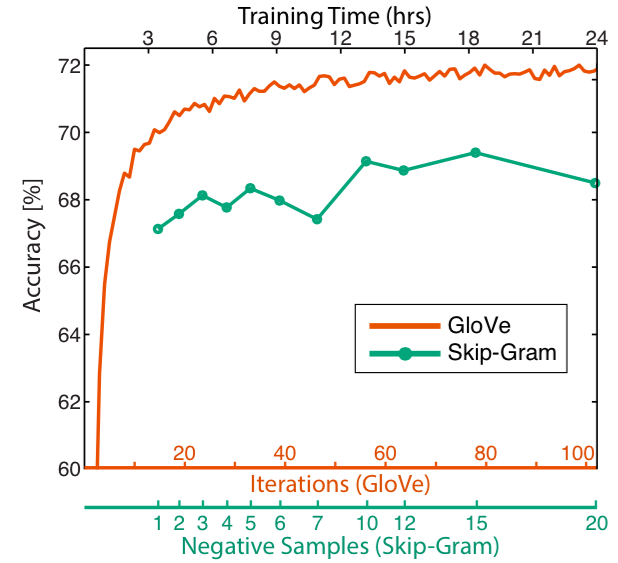
\includegraphics[width=\linewidth]{TrainTime}
  \caption{Here we see how training time improves training performance and helps squeeze the last few performance.}
  \label{fig:IntrinsicEval}
\end{marginfigure}


\item \textbf{Performance increases with larger corpus sizes:}\\ This happens because of the experience an embedding technique gains with more examples it sees. For instance, an analogy completion example will produce incorrect results if it has not encountered the test words previously.


\item \textbf{Performance is lower for extremely low as well as for extremely high dimensional word vectors:}\\ Lower dimensional word vectors are not able to capture the different meanings of the different words in the corpus. This can be viewed as a high bias problem where our model complexity is too low. For instance, let us consider the words "king", "queen", "man", "woman". Intuitively, we would need to use two dimensions such as "gender" and "leadership" to encode these into 2-bit word vectors. Any lower would fail to capture semantic differences between the four words and any more may capture noise in the corpus that doesn't help in generalization -- this is also known as the high variance problem.
\end{itemize}

Figure~\ref{fig:DataSize} demonstrates how accuracy has been shown to improve with larger corpus.

\begin{figure*}%
  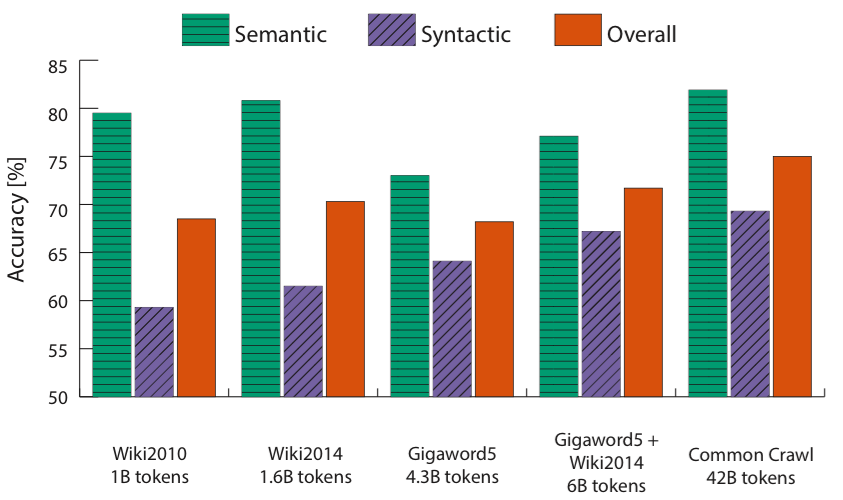
\includegraphics[width = 12cm]{DataSize}
  \caption{Here we see how performance improves with data size.}
  \label{fig:DataSize}
\end{figure*}

Figure~\ref{fig:hyperparam} demonstrates how other hyperparameters have been shown to affect the accuracies using GloVe.

\begin{figure*}%
  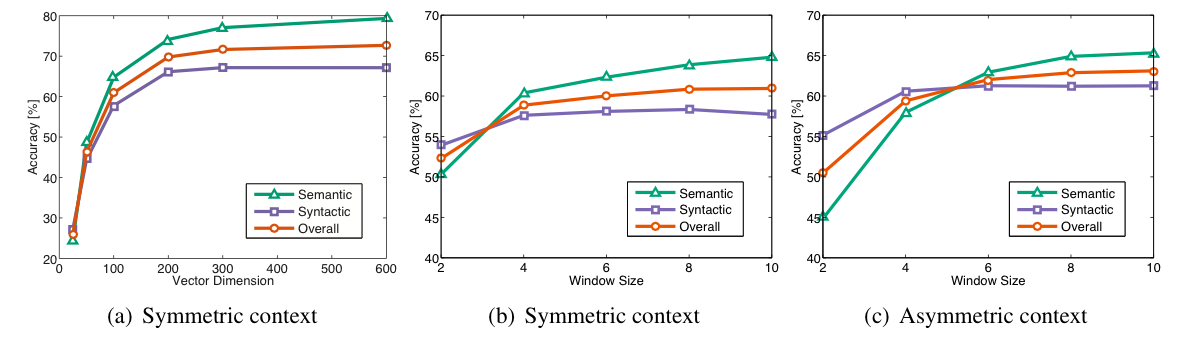
\includegraphics[width = 15cm]{hyperparam}
  \caption{We see how accuracies vary with vector dimension and context window size for GloVe}
  \label{fig:hyperparam}
\end{figure*}

\subsection{Intrinsic Evaluation Example: Correlation Evaluation}
Another simple way to evaluate the quality of word vectors is by asking humans to assess the similarity between two words on a fixed scale (say 0-10) and then comparing this with the cosine similarity between the corresponding word vectors. This has been done on various datasets that contain human judgement survey data.

\begin{table}[ht]
  \centering
  \fontfamily{ppl}\selectfont
  \begin{tabular}{ll | lllll}
    \toprule
    Model & Size & WS353 & MC & RG & SCWS & RW \\
    \midrule    
    SVD & 6B & 35.3 & 35.1 & 42.5 & 38.3 & 25.6\\
    SVD-S & 6B & 56.5 & 71.5 & 71.0 & 53.6 & 34.7\\
    SVD-L & 6B & 65.7 & 72.7 & 75.1 & 56.5 & 37.0\\
    CBOW & 6B & 57.2 & 65.6 & 68.2 & 57.0 & 32.5\\
    SG & 6B & 62.8 & 65.2 & 69.7 & 58.1 & 37.2\\
    GloVe & 6B & 65.8 & 72.7 & 77.8 & 53.9 & 38.1\\
    \hline
    SVD-L & 42B & 74.0 & 76.4 & 74.1 & 58.3 & 39.9\\
    GloVe & 42B & 75.9 & 83.6 & 82.9 & 59.6 & 47.8\\
    \hline
    CBOW & 100B & 68.4 & 79.6 & 75.4 & 59.4 & 45.5\\
    \bottomrule
  \end{tabular}
  \caption{Here we see the correlations between of word vector similarities using different embedding techniques with different human judgment datasets}
  \label{tab:normaltab}
\end{table}

\subsection{Further Reading: Dealing With Ambiguity}
One might wonder how we handle the situation where we want to capture the same word with different vectors for its different uses in natural language. For instance, "run" is both a noun and a verb and is used and interpreted differently based on the context. \textsc{Improving Word Representations Via Global Context And Multiple Word Prototypes (Huang et al, 2012)} describes how such cases can also be handled in NLP. The essence of the method is the following:

\begin{enumerate}
\item Gather fixed size context windows of all occurrences of the word (for instance, 5 before and 5 after)
\item Each context is represented by a weighted average of the context words' vectors (using idf-weighting)
\item Apply spherical k-means to cluster these context representations.
\item Finally, each word occurrence is re-labeled to its associated cluster and is used to train the word representation for that cluster.
\end{enumerate}

For a more rigorous treatment on this topic, one should refer to the original paper.

\section{Training for Extrinsic Tasks}

We have so far focused on intrinsic tasks and emphasized their importance in developing a good word embedding technique. Of course, the end goal of most real-world problems is to use the resulting word vectors for some other extrinsic task. Here we discuss the general approach for handling extrinsic tasks.

\subsection{Problem Formulation}
Most NLP extrinsic tasks can be formulated as classification tasks. For instance, given a sentence, we can classify the sentence to have positive, negative or neutral sentiment. Similarly, in named-entity recognition (NER), given a context and a central word, we want to classify the central word to be one of many classes. For the input, "Jim bought 300 shares of Acme Corp. in 2006", we would like a classified output "[Jim]\textunderscript{Person} bought 300 shares of [Acme Corp.]\textunderscript{Organization} in [2006]\textunderscript{Time}."

\begin{marginfigure}%
  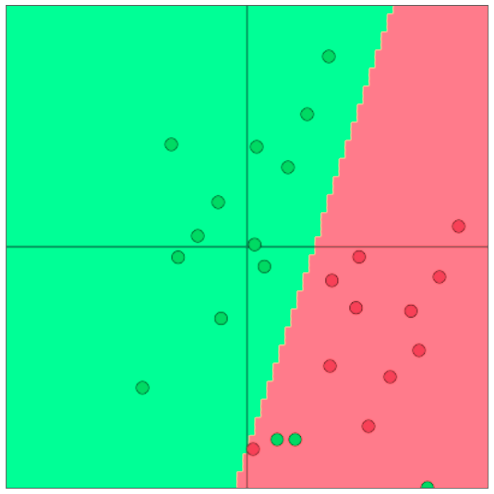
\includegraphics[width = \linewidth]{LinearBoundary}
  \caption{We can classify word vectors using simple linear decision boundaries such as the one shown here (2-D word vectors) using techniques such as logistic regression and SVMs}
  \label{fig:LinearBoundary}
\end{marginfigure}

For such problems, we typically begin with a training set of the form:
$$\{x^{(i)},y^{(i)}\}_1^N$$
where $x^{(i)}$ is a $d$-dimensional word vector generated by some word embedding technique and $y^{(i)}$ is a $C$-dimensional one-hot vector which indicates the labels we wish to eventually predict (sentiments, other words, named entities, buy/sell decisions, etc.).

In typical machine learning tasks, we usually hold input data and target labels fixed and train weights using optimization techniques (such as gradient descent, L-BFGS, Newton's method, etc.). In NLP applications however, we introduce the idea of retraining the input word vectors when we train for extrinsic tasks. Let us discuss when and why we should consider doing this.

\marginnote{\textbf{Implementation Tip:} Word vector retraining should be considered for large training datasets. For small datasets, retraining word vectors will likely worsen performance.}

\subsection{Retraining Word Vectors}

As we have discussed so far, the word vectors we use for extrinsic tasks are initialized by optimizing them over a simpler intrinsic task. In many cases, these pretrained word vectors are a good proxy for optimal word vectors for the extrinsic task and they perform well at the extrinsic task. However, it is also possible that the pretrained word vectors could be trained further (i.e. retrained) using the extrinsic task this time to perform better. However, retraining word vectors can be risky. 

\begin{marginfigure}%
  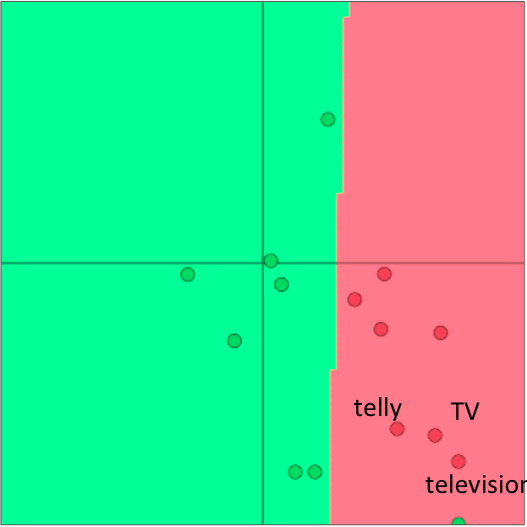
\includegraphics[width = \linewidth]{pretraining}
  \caption{Here, we see that the words "Telly", "TV", and "Television" are classified correctly before retraining. "Telly" and "TV" are present in the extrinsic task training set while "Television" is only present in the test set.}
    \label{fig:pretraining}
\end{marginfigure}

If we retrain word vectors using the extrinsic task, we need to ensure that the training set is large enough to cover most words from the vocabulary. This is because Word2Vec or GloVe produce semantically related words to be located in the same part of the word space. When we retrain these words over a small set of the vocabulary, these words are shifted in the word space and as a result, the performance over the final task could actually reduce. Let us explore this idea further using an example. Consider the pretrained vectors to be in a two dimensional space as shown in Figure~\ref{fig:pretraining}.  Here, we see that the word vectors are classified correctly on some extrinsic classification task. Now, if we retrain only two of those vectors because of a limited training set size, then we see in Figure~\ref{fig:retraining} that one of the words gets misclassified because the boundary shifts as a result of word vector updates.

Thus, word vectors should not be retrained if the training data set is small. If the training set is large, retraining may improve performance.

\begin{marginfigure}%
  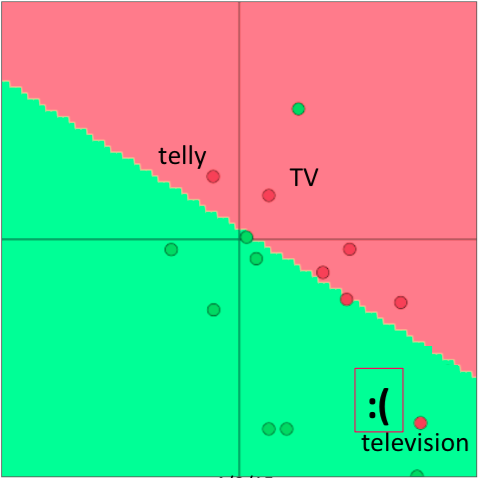
\includegraphics[width = \linewidth]{retraining}
  \caption{Here, we see that the words "Telly" and "TV" are classified correctly after traininng, but "Television" is not since it was not present in the training set.}
    \label{fig:retraining}
\end{marginfigure}

\subsection{Softmax Classification and Regularization}

Let us consider using the Softmax classification function which has the form:
$$p(y_j = 1|x) = \frac{\exp(W_{j\cdot}x)}{\sum_{c=1}^C\exp(W_{c\cdot}x)}$$
Here, we calculate the probability of word vector $x$ being in class $j$. Using the Cross-entropy loss function, we calculate the loss of such a training example as:
$$-\sum_{j=1}^{C}y_j\log(p(y_j = 1|x)) = -\sum_{j=1}^{C}y_j\log \bigg(\frac{\exp(W_{j\cdot}x)}{\sum_{c=1}^C\exp(W_{c\cdot}x)}\bigg)$$
Of course, the above summation will be a sum over $(C-1)$ zero values since $y_j$ is $1$ only at a single index (at least for now) implying that $x$ belongs to only $1$ correct class. Thus, let us define $k$ to be the index of the correct class. Thus, we can now simplify our loss to be:
$$-\log \bigg(\frac{\exp(W_{k\cdot}x)}{\sum_{c=1}^C\exp(W_{c\cdot}x)}\bigg)$$
We can then extend the above loss to a dataset of $N$ points:
$$-\sum_{i = 1}^N\log \bigg(\frac{\exp(W_{k{(i)}\cdot}x^{(i)})}{\sum_{c=1}^C\exp(W_{c\cdot}x^{(i)})}\bigg)$$
The only difference above is that $k(i)$ is now a function that returns the correct class index for example $x^{(i)}$.

Let us now try to estimate the number of parameters that would be updated if we consider training both, model weights ($W$), as well word vectors ($x$). We know that a simple linear decision boundary would require a model that takes in at least one $d$-dimensional input word vector and produces a distribution over $C$ classes. Thus, to update the model weights, we would be updating $C\cdot d$ parameters. If we update the word vectors for every word in the vocabulary $V$ as well, then we would be updating as many as $|V|$ word vectors, each of which is $d$-dimensional. Thus, the total number of parameters would be as many as $C\cdot d + |V|\cdot d$ for a simple linear classifier:

$$\nabla_{\theta} J(\theta) = \left[ \begin{array}{c} \nabla_{W_{\cdot 1}} \\  \vdots \\  \nabla_{W_{\cdot d}} \\ \nabla_{x_{aardvark}} \\ \vdots  \\ \nabla_{x_{zebra}} \end{array} \right] $$

This is an extremely large number of parameters considering how simple the model's decision boundary is - such a large number of parameters is highly prone to overfitting.

To reduce overfitting risk, we introduce a regularization term which poses the Bayesian belief that the parameters ($\theta$) should be small is magnitude (i.e. close to zero): 
$$-\sum_{i = 1}^N\log \bigg(\frac{\exp(W_{k{(i)}\cdot}x^{(i)})}{\sum_{c=1}^C\exp(W_{c\cdot}x^{(i)})}\bigg) + \lambda \sum_{k=1}^{C\cdot d + |V|\cdot d} \theta_k^2$$

Minimizing the above cost function reduces the likelihood of the parameters taking on extremely large values just to fit the training set well and may improve generalization if the relative objective weight $\lambda$ is tuned well. The idea of regularization becomes even more of a requirement once we explore more complex models (such as Neural Networks) which have far more parameters.

\subsection{Window Classification}

\begin{marginfigure}%
  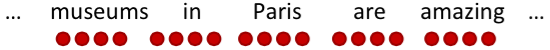
\includegraphics[width = \linewidth]{window}
  \caption{Here, we see a central word with a symmetric window of length 2. Such context may help disambiguate between the place Paris and the name Paris.}
    \label{fig:window}
\end{marginfigure}

So far we have primarily explored the idea of predicting in extrinsic tasks using a single word vector $x$. In reality, this is hardly done because of the nature of natural languages. Natural languages tend to use the same word for very different meanings and we typically need to know the context of the word usage to discriminate between meanings. For instance, if you were asked to explain to someone what "to sanction" meant, you would immediately realize that depending on the context "to sanction" could mean "to permit" or "to punish". In most situations, we tend to use a sequence of words as input to the model. A sequence is a central word vector preceded and succeeded by context word vectors. The number of words in the context is also known as the context window size and varies depending on the problem being solved. Generally, narrower window sizes lead to better performance in syntactic tests while wider windows lead to better performance in semantic tests.

\marginnote{Generally, narrower window sizes lead to better performance in syntactic tests while wider windows lead to better performance in semantic tests.}

In order to modify the previously discussed Softmax model to use windows of words for classification, we would simply substitute $x^{(i)}$ with  $x_{window}^{(i)}$ in the following manner:

$$x_{window}^{(i)} = \left[ \begin{array}{c} x^{(i-2)} \\ x^{(i-1)} \\ x^{(i)} \\ x^{(i+1)} \\ x^{(i+2)} \end{array} \right] $$

As a result, when we evaluate the gradient of the loss with respect to the words, we will receive gradients for the word vectors:

$$\delta_{window} = \left[ \begin{array}{c} \nabla_{x^{(i-2)}} \\ \nabla_{x^{(i-1)}} \\ \nabla_{x^{(i)}} \\ \nabla_{x^{(i+1)}} \\ \nabla_{x^{(i+2)}} \end{array} \right] $$

The gradient will of course need to be distributed to update the corresponding word vectors in implementation.

\subsection{Non-linear Classifiers}

\begin{marginfigure}%
  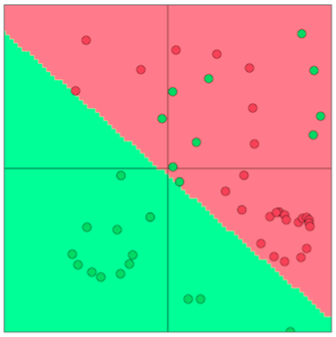
\includegraphics[width = \linewidth]{LinearBoundary2}
  \caption{Here, we see that many examples are wrongly classified even though the best linear decision boundary is chosen. This is due linear decision boundaries have limited model capacity for this dataset.}
    \label{fig:LinearBoundary2}
\end{marginfigure}

We now introduce the need for non-linear classification models such as neural networks. We see in Figure~\ref{fig:LinearBoundary2} that a linear classifier misclassifies many datapoints. Using a non-linear decision boundary as shown in Figure~\ref{fig:NonlinearBoundary}, we manage to classify all training points accurately. Although oversimplified, this is a classic case demonstrating the need for non-linear decision boundaries. In the next set of notes, we study neural networks as a class of non-linear models that have performed particularly well in deep learning applications.

\begin{marginfigure}%
  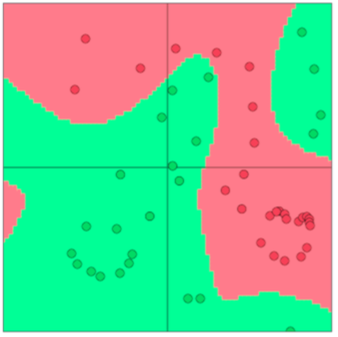
\includegraphics[width = \linewidth]{NonlinearBoundary}
  \caption{Here, we see that the non-linear decision boundary allows for much better classification of datapoints.}
    \label{fig:NonlinearBoundary}
\end{marginfigure}

\end{document}
